\chapter{Evaluation}

%In this chapter you should describe the previous (if possible) and final experiments performed on the implementation.

%Every single experiment should be explained individually, providing to the reader information about the meaning of the experiment, the expected %(theoretical) results, the final results, the comparison between them and others (if possible) and the conclusions. 

%Each experiment should include a description, covering (when possible) the following information:
%\begin{itemize}
%	\item Significant physical features (obstacles present on the environment, human presence, temperature, humidity, possible noise sources, computational speed of the machine, etc.)
%	\item The precise location of the experiment (latitude and longitude, room number or citation to a description of the used laboratory).
%	\item Sampling design (variable(s) measured, transformation performed to the data, samples collected, replication, comparative with a Ground Truth system, collecting data protocol).
%	\item Analysis design (how the data are processed, statistical procedures used, statistical level to determine significance).
%\end{itemize}
%The provided information should be sufficient to allow other scientists to repeat your experiment in the same conditions. Thus, the use of standard and %well-known equipment could only be represented by a simple sentence, but the non-standard equipment should be described in detail, citing the source %(vendor) and most important characteristics.

%To write it, try to use the third person when describing the experiments and results. Avoid to use first person. Past tense should be the dominant %conjugation (the work is done and was performed in the past).

%Note: Graphics represent really well data, use them! (Matlab or Octave could be useful for that).

\section{Experiment Setup}
To test the suggested approach for a RSS measurement system described in Chapter \ref{chp:apr} the approach was implemented like described in Chapter \ref{chp:imp}. System was then deployed and tested inside the Testbed described in Chapter \ref{chp:mat_testbed}. Two experiments where run. The first one was at night where no one was inside the building where the Testbed is located. The second one was at daytime when there where people where working inside the offices covered by the Testbed and also in the other parts of the building. 

The implemented system still had some bugs that could not be addressed due to lack of time. However these bugs only made the system stop at one point during the collection and did not influence the measured times for the different phases. This made it necessary to start the system multiple times for each experiment. The application was restarted after half an hour to catch stops. This however made it impossible to evaluate how long it takes until a new calibration is needed.

To calibrate the system 700 messages were sent with a minimum break of 20 ms. After the sink send all its messages it takes a 50 second break to make sure every node send its message. The timeslot for the drops was defined as 18 ms. This is really big but when running the system inside a simulation it could be measured that the processing and sending of a message took between 5 ms and 16 ms the extra 2 ms cover a possible error while measuring these values.  
\section{Experiment Night}
The first experiment took place at night between 02:00h and 05:30h. At this time no one was present at the whole floor. In this time system was started and restarted 7 times. Between 03:30 and 04:30 the application actually ran the whole 30 minutes and was not stopped by the bug but by the next restart. In all the other cases the application stopped during a collection. In Table \ref{tab:NightTable} the times for each start of the application a shown as well as the over all average times for each phase. 

\begin{table}[htbp]
 \caption{Measured values for each run of the system. CT = Calibration Times; HOP = Number of hops inside the schedule; ST = Spread time; ACT = Average collection time; CSTD = Standard deviation of collection time; ART = Average round time; RSTD = Standard deviation of round time;}
 \centering
 \begin{tabular}{c||c|c|c|c|c|c|c|c}
  Time & CT & HOP & ST & ACT & CSTD & ART & RSTD & Rounds\\ \toprule
  02:00 - 02:30 & 65611 & 44 & 784 & 3592 & 267 & 540 & 55 & 338\\
  02:30 - 03:00 & 64545 & 42 & 842 & 3637 & 280 & 519 & 38 & 73\\
  03:00 - 03:30 & 64630 & 42 & 767 & 4211 & 444 & 502 & 32 & 13\\
  03:30 - 04:00 & 64539 & 41 & 740 & 3609 & 300 & 501 & 62 & 420\\
  04:00 - 04:30 & 64565 & 44 & 804 & 3581 & 245 & 544 & 51 & 419\\
  04:30 - 05:00 & 64699 & 40 & 756 & 4287 & 343 & 429 & 48 & 35\\
  05:00 - 05:30 & 64587 & 44 & 787 & 4150 & 343 & 496 & 23 & 9\\ \toprule
  Average & 64739 & 42 & 782 & 3625 & 276 & 524 & 54 & \\
 \end{tabular}
 \label{tab:NightTable}
\end{table}

The average calibration time was 64739 ms. The time of all the different calibrations did not really change since the exact amount of messages and the break between messages is defined. It takes quite long since a huge amount of messages are send by each node with a break up to 32 ms. Also the break the sink takes after it send its message was not calculated perfectly making it possible to reduce resulting in a shorter calibration. When the calibration phase took roughly 64 seconds and the sink took a 50 second it means the sink was done after 14 seconds. Now with the defined break for all the nodes in Chapter (imp szutt) we can calculate the maximum time a node needs to send all its messages. The result would be that the node would take around 40 seconds. This means the calibration time could be reduced by 20 seconds when calculating a correct break for the sink.

The average schedule has 42 hops meaning that 42 messages need to be send in one round the schedule takes. The schedule with the largest amount of hops has 44 and the smallest has 40 hops. The different schedules emerge through different measured RSS values while calibrating.

Spreading the schedule took averagely 782 ms. This is really fast since one schedule of 40+ hops needs two messages. This means that to spread one schedule part inside the whole network took around 370 ms.

The collection of the gathered information took averagely 3625 ms with an average standard deviation of 276 ms. Compared with the spreading of the schedule this is really slow. However we need to take into account that the collection takes a lot more messages and processing than the spreading. To analyse if the time of the collection changes during the curse of time and if a new calibration is needed. Figure \ref{fig:nightC} shows the times of all the collections between 03:30h and 04:00h. However the Figure does not show any significant change over the 30 minutes of time indicating that there would be no new calibration necessary to maintain the highest possible performance of the application.

\begin{figure}[htbp]
	\centering         
    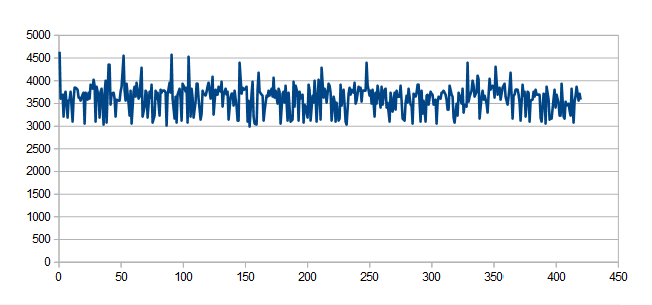
\includegraphics[scale=0.75]{content/images/Experiment/NightCollection}
    \caption{Collection times of the measurements from 03:30h to 04:00h}
	\label{fig:nightC}
\end{figure}

Sending all the messages for one round takes averagely 524 ms with a average standard deviation of 54 ms. Again we want to analyse if the time changes during the curse of time. Therefore the times of all the rounds between 03:30h and 04:00h are shown in Figure \ref{fig:nightR}. Again we do not see a significant change in the time one round takes. This means that message drops to not increase making the measurements still usable for localisation.

\begin{figure}[tbp]
	\centering
	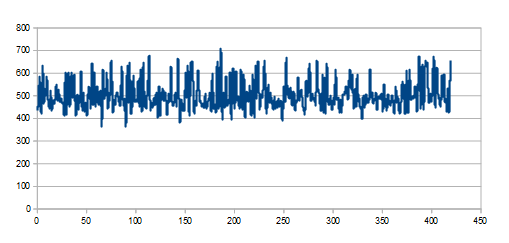
\includegraphics[scale=0.75]{content/images/Experiment/NightRounds}
 	\caption{Sampling times of the measurements from 03:30h to 04:00h}
	\label{fig:nightR}
\end{figure}

\section{Experiment Day}
The second experiment took place from 09:15h to 12:45h. In this timespan the application was started and restarted 9 times. The first person arrived at 10:00h, the second at 11:20h, the third at 13:00h and the last one at 13:30. Moreover one person arrived and left somewhere between 10:30h and 12:30h. All these people where working in their offices.
The results of the experiment are shown in Table \ref{tab:DayTable}
\begin{table}[htbp]
 \caption{Measured values for each run of the system. CT = Calibration Times; HOP = Number of hops inside the schedule; ST = Spread time; ACT = Average collection time; CSTD = Standard deviation of collection time; ART = Average round time; RSTD = Standard deviation of round time;}
 \centering
 \begin{tabular}{c|c||c|c|c|c|c|c|c|c}
  Time & Persons & CT & HOP & ST & ACT & CSTD & ART & RSTD & Rounds\\ \toprule
  09:15 - 09:45 & 0 & 64647 & 43 & 823 & 4401 & 296 & 492 & 41 & 63\\ 
  09:45 - 10:15 & 1 & 64558 & 44 & 796 & 4035 & 322 & 563 & 59 & 121\\
  10:15 - 10:45 & 1 & 64644 & 41 & 850 & 3740 & 282 & 482 & 40 & 231\\
  10:45 - 11:15 & 1 & 64577 & 41 & 849 & 3746 & 423 & 533 & 60 & 14\\ 
  11:15 - 11:45 & 2 & 64607 & 39 & 797 & 3498 & 358 & 495 & 42 & 433\\
  11:45 - 12:15 & 2 & 64654 & 41 & 764 & 3556 & 294 & 495 & 45 & 240\\
  12:15 - 12:45 & 2 & 64583 & 44 & 824 & 4160 & 511 & 539 & 65 & 368\\
  12:45 - 13:15 & 3 & 64544 & 44 & 797 & 3697 & 398 & 542 & 58 & 183\\
  13:15 - 13:45 & 4 & 64580 & 41 & 778 & 3494 & 371 & 528 & 46 & 73\\ \toprule
  Average & & 64599 & 42 & 809 & 3773 & 372 & 514 & 50 & \\
 \end{tabular}
 \label{tab:DayTable}
\end{table}

All the values are not significantly different to the values at night. Again we look at the individual times of the collection in Figure \ref{fig:dayC} to see if they change over time. In general the time for a collection does not increase over time, however at around collection 400 we can see a huge eruption. Here the collection once takes 5186 ms and once
7293 ms. After that the collection time normalizes again. This eruption could indicate that at that point in time a, for the links inside the Tesbed, huge change in the environment caused a lot of message drops creating this long collection. This could be an open door that has not been open before or maybe someone calling the elevator and going down with it. 


\begin{figure}[htbp]
	\centering         
    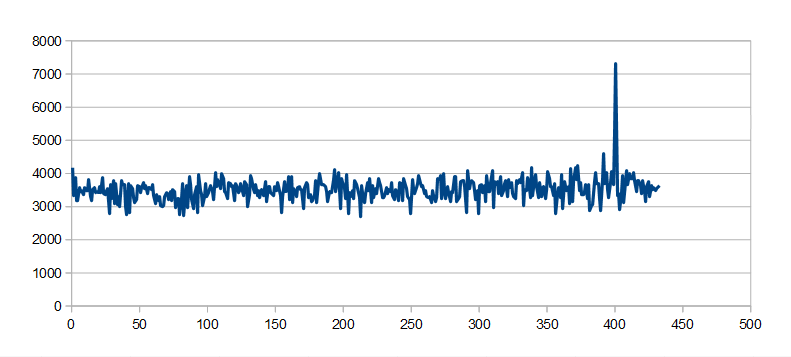
\includegraphics[scale=0.75]{content/images/Experiment/DayCollection}
    \caption{Collection times of the measurements from 03:30h to 04:00h}
	\label{fig:dayC}
\end{figure}



\begin{figure}[tbp]
	\centering
    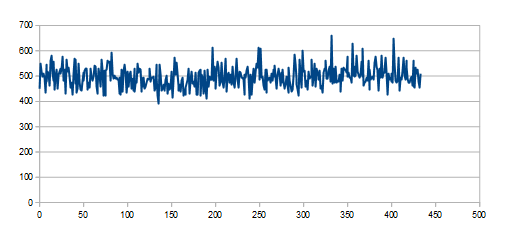
\includegraphics[scale=0.75]{content/images/Experiment/DayRounds}
   	\caption{Sampling times of the measurements from 03:30h to 04:00h}
    \label{fig:DayR}
\end{figure}
    

\section{Assessment}